\chapter{微服务部署与验证}
\section{Kubernetes环境搭建}
为了成功部署和管理云原生微服务应用,我们需要建立一个可靠的Kubernetes集群环境。本节将简要介绍Kubernetes环境搭建的步骤,并提供系统参数配置示例。

参考本实验所使用的Kubernetes集群环境如下表所示:

\begin{table}[ht]\centering
\begin{tabular}{l|l|l}
	\hline\hline
	虚拟机hostname        & IP地址&含义              \\ \hline
	master&192.168.210.128&Kubernetes集群主节点,应用部署端,服务监控端 \\ \hline
	node1&192.168.210.129& Kubernetes集群从节点1\\ \hline
	node2&192.168.210.130& Kubernetes集群从节点2\\ 
\hline\hline
\end{tabular}
\end{table}
\subsection{虚拟机节点准备}
在开始搭建Kubernetes集群之前,确保所有虚拟客户机满足Kubernetes的最低硬件要求,并选择适合的操作系统版本。本实验使用稳定的Linux发行版CentOS 7.9,每台机器 8 GB 内存,2核4个CPU,集群中的所有机器的网络彼此均能相互连接,节点中无有重复的主机名、MAC 地址或 product\_uuid。对集群中的每台虚拟机,执行如下指令,关闭 SELinux、关闭防火墙、关闭swap分区:
\begin{lstlisting}[language=bash]
systemctl stop firewalld
systemctl disable firewalld
vim /etc/selinux/config
setenforce 0
swapoff -a
vim /etc/fstab
#注释swap
\end{lstlisting}
添加域名映射,测速节点之间是否能互相Ping:
\begin{lstlisting}[language=bash]
vim /etc/hosts
192.168.210.128 master
192.168.210.129 node1
192.168.210.130 node2
\end{lstlisting}
同步网络时间后,为三台虚拟机都添加阿里源,以绕过翻墙或下载速度过慢。
\begin{lstlisting}[language=bash]
cat <<EOF > /etc/yum.repos.d/kubernetes.repo
[kubernetes]
name=Kubernetes
baseurl=http://mirrors.aliyun.com/kubernetes/yum/repos/kubernetes-el7-x86_64
enabled=1
gpgcheck=1
repo_gpgcheck=0
gpgkey=http://mirrors.aliyun.com/kubernetes/yum/doc/yum-key.gpg http://mirrors.aliyun.com/kubernetes/yum/doc/rpm-package-key.gpg
EOF
\end{lstlisting}
为了正确配置系统参数,创建并编辑文件\texttt{/etc/sysctl.d/k8s.conf},将以下内容添加到文件中:
\begin{lstlisting}[language=bash]
net.bridge.bridge-nf-call-ip6tables=1
net.bridge.bridge-nf-call-iptables=1
net.ipv4.ip_forward=1
vm.swappiness=0
\end{lstlisting}

然后,通过运行命令\texttt{sysctl --system}使参数生效。

\subsection{为所有节点安装Docker}
Kubernetes使用Docker容器来运行应用程序。在所有节点上安装Docker,并根据实际需求进行配置。首选,添加docker的yum源:

\begin{lstlisting}[language=bash]
yum-config-manager --add-repo https://download.docker.com/linux/centos/docker-ce.repo
yum -y install docker-ce-20.10.9 docker-ce-cli-20.10.9 containerd.io
systemctl enable docker
systemctl start docker
\end{lstlisting}
接下来,编辑文件\texttt{/etc/docker/daemon.json},将以下内容添加到文件中:
\begin{lstlisting}[language=bash]
{
"registry-mirrors": ["https://b9pmyelo.mirror.aliyuncs.com"],
"exec-opts": ["native.cgroupdriver=systemd"]
}
\end{lstlisting}

此处,需要注意的是对\texttt{exec-opt}的修改:参考\citep{systemd},cgroups(Control Groups) 是 linux 内核提供的一种机制,它可以限制、记录任务组所使用的物理资源,是内核附加在程序上的hook,使程序运行时对资源的调度触发相应的钩子,达到资源追踪和限制资源使用的目的。Kubernetes 推荐使用 systemd 来代替 cgroupfs,因为systemd是Kubernetes自带的cgroup管理器, 负责为每个进程分配cgroups, 但docker的cgroup driver默认是cgroupfs,这样就同时运行有两个cgroup控制管理器, 当资源有压力的情况时,有可能出现不稳定的情况。最后,通过运行命令\texttt{systemctl restart docker}使配置生效。


\subsection{为所有节点安装Kubernetes}
首先,创建并编辑文件\texttt{/etc/yum.repos.d/kubernetes.repo},将以下内容添加到文件中:
\begin{lstlisting}[language=bash]
[kubernetes]
name = Kubernetes
baseurl = https://mirrors.aliyun.com/kubernetes/yum/repos/kubernetes-el7-x86_64
enabled = 1
gpgcheck = 0
repo_gpgcheck = 0
gpgkey = https://mirrors.aliyun.com/kubernetes/yum/doc/yum-key.gpg
https://mirrors.aliyun.com/kubernetes/yum/doc/rpm-package-key.gpg
\end{lstlisting}

然后,运行以下命令安装Kubernetes组件:
\begin{lstlisting}[language=bash]
yum -y install kubelet-1.22.6 kubeadm-1.22.6 kubectl-1.22.6
systemctl enable kubelet
\end{lstlisting}

\subsection{集群master节点初始化与node节点加入}
使用以下命令初始化Kubernetes集群:
\begin{lstlisting}[language=bash]
kubeadm init \
--apiserver-advertise-address=192.168.210.128 \
--image-repository registry.aliyuncs.com/google_containers \
--kubernetes-version v1.22.6 \
--service-cidr=10.96.0.0/12 \
--pod-network-cidr=10.244.0.0/16
\end{lstlisting}

在初始化完成后,创建存储Kubernetes配置文件的目录,然后,将管理员配置文件复制到用户目录,并设置正确的权限:
\begin{lstlisting}[language=bash]
mkdir -p $HOME/.kube
sudo cp -i /etc/kubernetes/admin.conf $HOME/.kube/config
sudo chown $(id -u):$(id -g) $HOME/.kube/config
\end{lstlisting}

使用以下命令将节点加入Kubernetes集群:
\begin{verbatim}
kubeadm join 192.168.210.128:6443 --token s19psv.t5r2ms4sos28duxc \
--discovery-token-ca-cert-hash sha256:21d529dc1ac201206aa4c0a417982bbd9561ad06e2ee34302205c51a482b7bb4
\end{verbatim}
通过执行上述命令,将节点成功加入到Kubernetes集群中。

\subsection{网络配置}
为Kubernetes集群配置网络,确保各个节点之间可以通信,并提供外部访问服务的能力。本实验采取falnnel网络插件,使用离线安装:
\begin{lstlisting}[language=bash]
kubectl apply -f kube-flannel.yml
\end{lstlisting}

\subsection{Kubernetes集群配置结果}
节点成功加入Kubernetes集群的标志是通过执行以下命令后,在输出中看到类似以下信息:
\begin{verbatim}
This node has joined the cluster:
* Certificate signing request was sent to apiserver and a response was received.
* The Kubelet was informed of the new secure connection details.
\end{verbatim}

执行 \texttt{kubectl get nodes} 命令,检查新加入的节点是否以 Ready 状态显示。
\begin{figure}[htb]
\centering
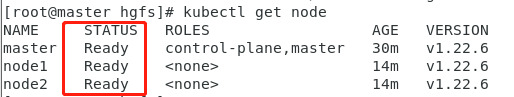
\includegraphics[width=1.0\textwidth]{figures/chapter2/getnode.png}
\caption{Kubernetes集群搭建成功后节点状态}
\label{fig:Kubernetes集群搭建成功后节点状态}
\end{figure}
至此Kubernetes集群环境搭建完毕,master作为master节点,node1,node2作为worker节点。
\begin{table}[ht]\centering
\begin{tabular}{l|l|l|l}
	\hline\hline
	服务器& 操作系统版本&	CPU架构&	功能描述\\ \hline
	master/192.168.210.128&CentOS Linux7.9&	x86\_64&k8s master节点 \\ \hline
	node1/192.168.210.129& CentOS Linux7.9&x86\_64&k8s worker节点\\ \hline
	node2/192.168.210.130& CentOS Linux7.9&x86\_64&k8s worker节点\\ 
	\hline\hline
\end{tabular}
\caption{Kubernetes集群架构}
\end{table}
\section{Kubernetes Dashboard部署}
Dashboard是一个Kubernetes集群的可视化管理工具,可以通过Web界面直观地查看和管理集群中的资源。根据兼容性要求,确认所使用的Dashboard版本与Kubernetes版本匹配。可以参考兼容性参考文档:\url{https://github.com/kubernetes/dashboard}。本实验分如下步骤搭建Dashboard环境:
使用下载好的kubernetes-dashboard-v2.0.3.yml配置文件进行安装,修改YAML文件,将Service的类型(type)修改为NodePort,并将端口(port)设置为31260。在文件的40行和44行进行修改。用kubectl命令apply -f即可。
\begin{lstlisting}[language=bash]
kubectl apply -f kubernetes-dashboard-v2.0.3.yml
\end{lstlisting}
使用以下命令验证Dashboard的Pod状态是否为Running:
\begin{lstlisting}[language=bash][language=bash]
kubectl get pod --namespace=kubernetes-dashboard -o wide | grep dashboard
\end{lstlisting}
创建Dashboard的访问权限:
\begin{lstlisting}[language=bash]
kubectl apply -f create-admin.yaml
\end{lstlisting}
其中,\texttt{create-admin.yaml}是一个包含访问权限配置的YAML文件.
获取Dashboard的访问地址:
\begin{lstlisting}[language=bash]
kubectl -n kubernetes-dashboard describe service kubernetes-dashboard
\end{lstlisting}
在输出中,找到 \texttt{LoadBalancer Ingress} 字段下的IP地址和端口号,即可访问Dashboard的Web界面。
查看Dashboard的服务端口,可以使用以下命令:
\begin{lstlisting}[language=bash]
kubectl get service -n kube-system | grep dashboard
\end{lstlisting}
确认端口号为30001。
打开Web浏览器,输入访问地址,在登录界面中选择"Token"认证方式,并将上一步中获取到的Token粘贴到相应的输入框中。并使用之前设置的访问权限进行登录。
\begin{figure}[htb]
\centering
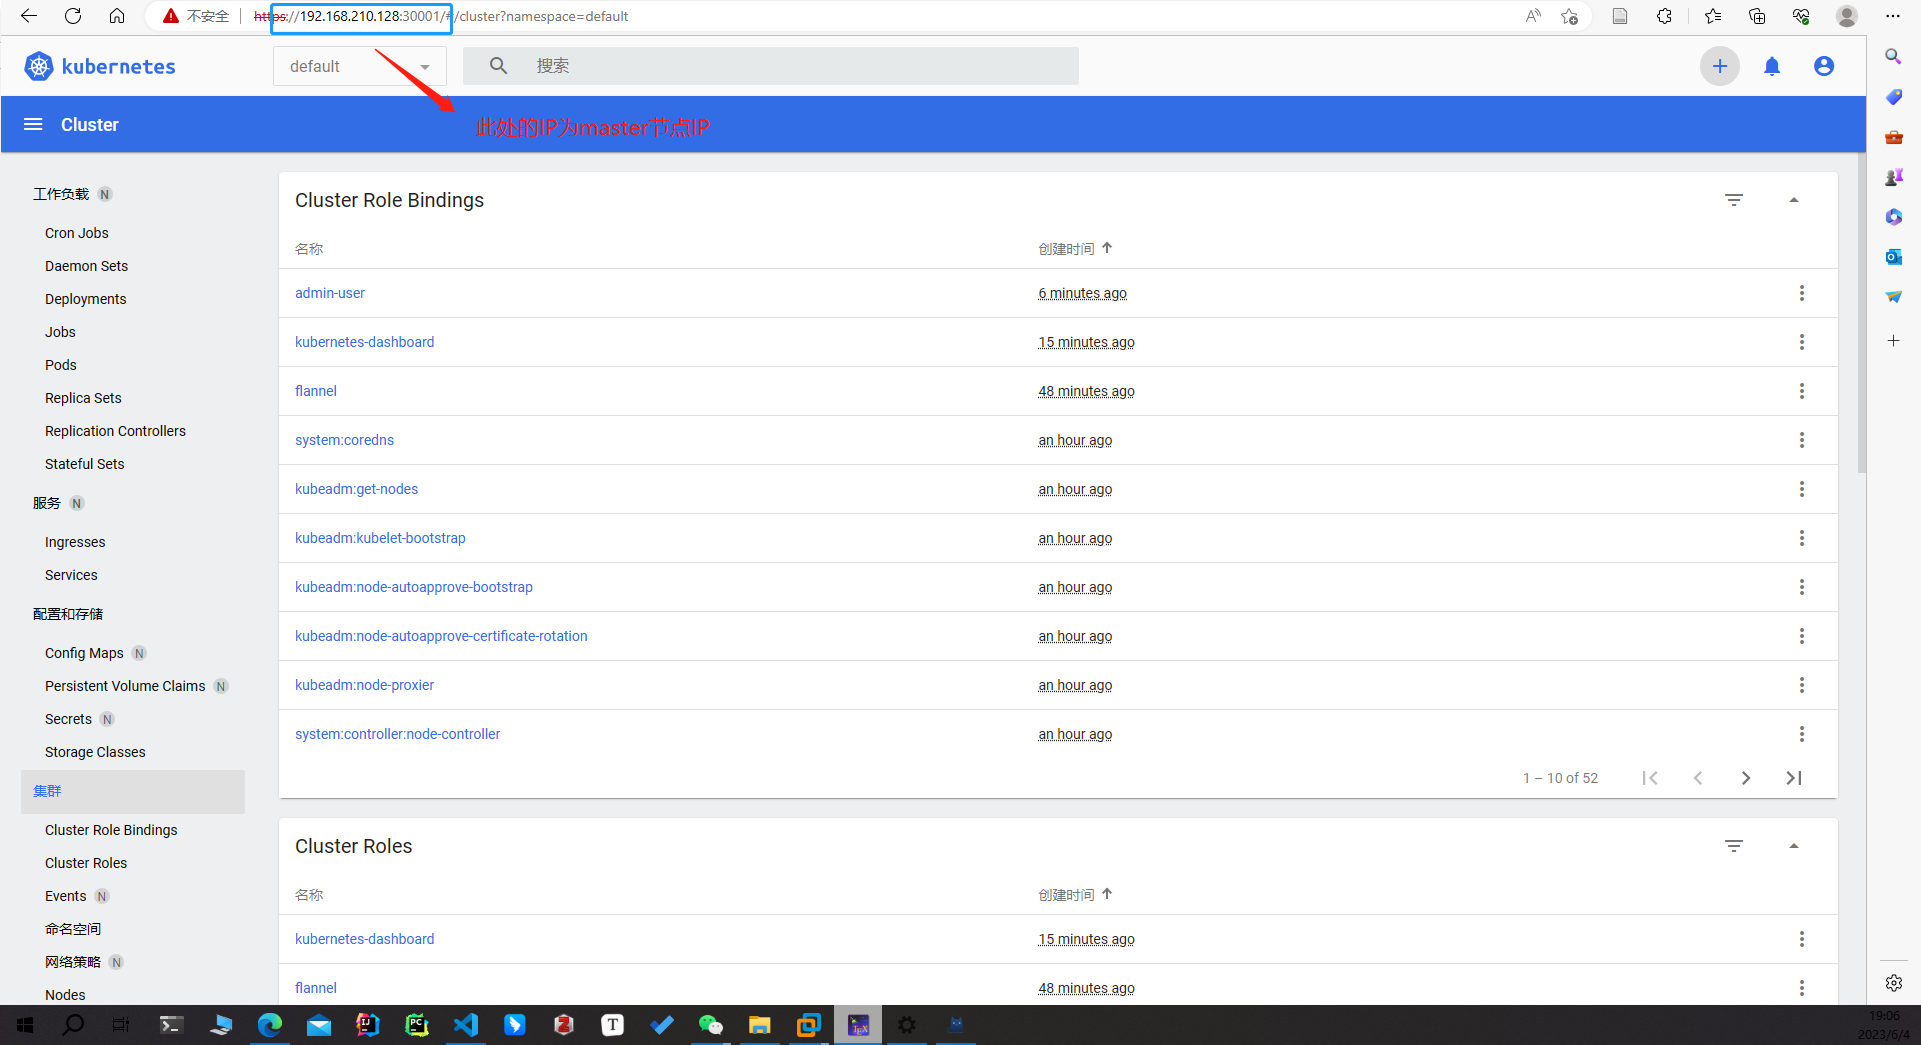
\includegraphics[width=1.0\textwidth]{figures/chapter2/dashboard.png}
\caption{Kubernetes Dashboard登录后的集群展示界面}
\label{fig2:Kubernetes Dashboard登录后的集群展示界面}
\end{figure}

\section{Istio与Online-Boutique项目微服务部署}
\subsection{单体架构与微服务架构}
在软件设计中,经常提及和使用经典的3层模型,即表示层、业务逻辑层和数据访问层。
\begin{itemize}
	\item 表示层:用于直接和用户交互,也称为交互层,通常是网页、UI 等。
	
	\item 业务逻辑层:即业务逻辑处理层,例如用户输入的信息要经过业务逻辑层的处理后,才能展现给用户。
	
	\item 数据访问层:用于操作数据库,用户在表示层会产生大量的数据,通过数据访问层对数据库进行读写操作。
\end{itemize}

虽然在软件设计中划分了经典的3层模型,但是对业务场景没有划分。一个典型的单体应用就是将所有的业务场景的表示层、业务逻辑层和数据访问层放在一个工程中,最终经过编译、打包,部署在一台服务器上。

单体架构部署简单,可以直接部署在一个服务器上即可。使用技术单一,项目不需要复杂的技术栈,往往一套熟悉的技术栈就可以完成开发,而且用人成本低 单个程序员可以完成业务接口到数据库的整个流程。但是也有一定缺陷,例如:
\begin{itemize}
	\item 系统启动慢 , 一个进程包含了所有的业务逻辑,涉及到的启动模块过多,导致系统的启动、重启时间周期过长
	
	\item 系统错误隔离性差、可用性差,任何一个模块的错误均可能造成整个系统的宕机
	
	\item 可伸缩性差;系统的扩容只能只对这个应用进行扩容,不能做到对某个功能点进行扩容
	
	\item 线上问题修复周期长;任何一个线上问题修复需要对整个应用系统进行全面升级
\end{itemize}

微服务架构风格\cite{weifuwujiagou}是一种将一个单一应用程序开发为一组小型服务的方法每一个服务运行在自己的进程中服务间通信采用的轻量级通信机制通(常用HTTP 资源 API ). 这些服务围绕业务能力构建并且可通过全自动部署机制独立部署这些服务公用一个最小型的集中式的管理服务可用不同的语言开发,使用不同的数据存储技术。

微服务架构以其易于开发和维护的特性受到广泛关注。每个微服务专注于特定的业务功能,使得业务清晰,代码量少。开发和维护单个微服务相对简单,而整个应用由多个微服务构建,使整体应用保持可控状态。此外,微服务的启动速度快,因为每个微服务的代码量较少。相比于单体架构模式,微服务解决了整个应用修改后重新部署的问题。一般情况下,对某个微服务进行修改只需要重新部署该服务即可。

在微服务架构中,可以根据项目业务和团队特点,灵活选择技术栈。不同的微服务可以使用适合的技术工具,例如关系型数据库MySQL或非关系型数据库Redis。此外,根据需求,部分微服务可以使用Java开发,而其他微服务则可以选择Node.js开发。这种灵活性使得微服务架构更加适应各种项目需求。

另外,微服务架构支持按需收缩,实现细粒度的扩展。例如,当某个微服务遇到瓶颈时,可以根据该微服务的业务特点,增加内存、升级CPU或增加节点等方式进行扩展,以满足系统的需求。

通过微服务架构,我们可以充分利用其优势,使得开发和维护变得简单高效。同时,根据项目需求和团队特点,选择适合的技术工具和灵活扩展方式,为应用提供高度可定制的解决方案。

\subsection{Online Boutique 代码分析}
Online Boutique由11个使用不同编程语言编写的微服务组成,它们通过gRPC进行相互通信。在./protos目录下可以找到协议缓冲描述。具体地,Online Boutique 由以下微服务组成:

\begin{tabularx}{\textwidth}{|l|l|X|}
	\hline
	\textbf{服务} & \textbf{编程语言} & \textbf{描述} \\
	\hline
	前端服务 & Go & 提供一个HTTP服务器来提供网站。无需注册/登录,自动生成所有用户的会话ID。 \\\hline
	购物车服务 & C\# & 将用户的购物车项目存储在Redis中并检索它。 \\\hline
	产品目录服务 & Go & 从JSON文件中提供产品列表,并能够搜索产品和获取单个产品的详细信息。 \\\hline
	货币转换服务 & Node.js & 将一个货币金额转换为另一种货币。使用从欧洲央行获取的实时数据。这是最高请求量的服务。 \\\hline
	支付服务 & Node.js & 使用给定的信用卡信息(模拟)对给定金额进行扣款,并返回交易ID。 \\\hline
	配送服务 & Go & 根据购物车提供运费估算,并将商品运送到指定地址(模拟)。 \\\hline
	邮件服务 & Python & 向用户发送订单确认邮件(模拟)。 \\\hline
	结账服务 & Go & 检索用户的购物车,准备订单,并协调支付、配送和邮件通知。 \\\hline
	推荐服务 & Python & 基于购物车内容推荐其他产品。 \\\hline
	广告服务 & Java & 根据给定的上下文词汇提供文本广告。 \\\hline
	负载生成器 & Python/Locust & 使用Locust负载生成器模拟真实用户的购物流程连续发送请求给前端。 \\
	\hline
\end{tabularx}
该项目具有以下特征:
\begin{itemize}
	\item Kubernetes/GKE:该应用程序设计为在Kubernetes上运行(包括本地的“Docker for Desktop”和云端的GKE)。
	\item gRPC:微服务之间使用大量的gRPC调用进行通信。
	\item Istio:应用程序在Istio服务网格上运行。
	\item Cloud Operations(Stackdriver):许多服务都使用了性能分析和跟踪功能。此外,使用Istio还可以获得请求/响应指标和上下文图等功能。当应用程序在Google Cloud之外运行时,这些代码路径将处于非活动状态。
	\item Skaffold:使用Skaffold命令将应用程序一键部署到Kubernetes。
	\item 合成负载生成:该应用程序演示了使用Locust负载生成器创建真实使用模式的背景作业。
\end{itemize}
\subsection{安装Istio}
本实验采用的 Istio 的版本为 1.5.7,首先检查集群是否正常。

\begin{lstlisting}[language=bash]
[root@master ~]# kubectl get node
NAME         STATUS   ROLES                  AGE    VERSION
master   Ready    control-plane,master   288d   v1.21.9
node1   Ready    <none>                 288d   v1.21.9
node2   Ready    <none>                 288d   v1.21.9
\end{lstlisting}

本实验安装 Istio 的 demo 配置文件,因为它包含所有的核心组件,并启用了跟踪和日志记录,便于学习不同的 Istio 功能,该过程主要参考博客\cite{istio},但后来部署项目时发现问题,主要是Gateway与HTTPRouter两个kind的问题,于是参考Stackoverflow中的回答\footnote{\url{https://stackoverflow.com/questions/69461513/no-matches-for-kindgateway-and-virtualservice}},下载了crd-all.gen.yaml并执行安装。

\begin{lstlisting}[language=bash][language=bash]
# 下载 GetMesh CLI
curl -sL https://istio.tetratelabs.io/getmesh/install.sh | bash

# 安装 Istio
getmesh istioctl install --set profile=demo
kubectl apply -f ./crd-all.gen.yaml
\end{lstlisting}
\subsection{Online Boutique 应用部署}
Istio 安装完成后,创建一个名为 \texttt{online-boutique} 的命名空间,新的项目将部署在该命名空间下,并为命名空间设置 \texttt{istio-injection=enabled} 标签,以启用 Sidecar 自动注入。

\begin{lstlisting}[language=bash][language=bash]
# 创建命名空间 online-boutique
[root@master ~]# kubectl create ns online-boutique
namespace/online-boutique created

# 切换命名空间
[root@master ~]# kubens online-boutique
Context "kubernetes-admin@kubernetes" modified.
Active namespace is "online-boutique".

# 让命名空间 online-boutique 启用 Sidecar 自动注入
[root@master ~]# kubectl label ns online-boutique istio-injection=enabled
namespace/online-boutique labeled

[root@master ~]# kubectl get ns -l istio-injection --show-labels
NAME              STATUS   AGE   LABELS
online-boutique   Active   16m   istio-injection=enabled,kubernetes.io/metadata.name=online-boutique
\end{lstlisting}

为了克隆代码仓库,我们需要安装Git,并执行以下命令:

\begin{lstlisting}[language=bash]
[root@master ~]# yum -y install git
[root@master ~]# git version
git version 1.8.3.1
[root@master ~]# mkdir online-boutique
[root@master ~]# cd online-boutique/
[root@master online-boutique]# git clone https://github.com/GoogleCloudPlatform/microservices-demo.git
\end{lstlisting}

在克隆完成后,进入\texttt{microservices-demo}目录,其中\texttt{istio-manifests.yaml}和\texttt{kubernetes-manifests.yaml}是主要的安装文件。

\begin{lstlisting}[language=bash]
[root@master online-boutique]# cd microservices-demo/
[root@master microservices-demo]# ls
cloudbuild.yaml     CODEOWNERS       docs  istio-manifests       kustomize  pb         release        SECURITY.md    src
CODE_OF_CONDUCT.md  CONTRIBUTING.md  hack  kubernetes-manifests  LICENSE    README.md  renovate.json  skaffold.yaml  terraform
\end{lstlisting}

\subsection{镜像构建}
在部署 Online Boutique 应用时,我们可以看到在 kubernetes-manifests.yaml 文件中列出了应用所需的 13 个镜像。这些镜像包括了 Google 提供的一些服务和应用组件,其镜像名称以 gcr.io 开头。为了提高镜像下载速度,我们可以将这些镜像地址中的 gcr.io 替换为 gcr.lank8s.cn,以便从国内的镜像源进行下载。在集群的工作节点上使用以下命令来提前下载镜像。以 node1 节点为例,执行以下命令:
\begin{lstlisting}[language=bash]
[root@node1 ~]# docker pull gcr.lank8s.cn/google-samples/microservices-demo/emailservice:v0.7.0
。。。。。。
% 其他那些镜像就按照此方法下载......
。。。。。。
[root@node1 ~]# docker pull gcr.lank8s.cn/google-samples/microservices-demo/adservice:v0.7.0
\end{lstlisting}
使用\texttt{sed -i 's/gcr.io/gcr.lank8s.cn/' kubernetes-manifests.yaml}修改镜像地址, gcr.io 替换为 gcr.lank8s.cn
\begin{lstlisting}[language=bash]
% 此时kubernetes-manifests.yaml文件中的镜像就全被修改了
[root@master release]# grep image kubernetes-manifests.yaml
image: gcr.lank8s.cn/google-samples/microservices-demo/emailservice:v0.4.0
image: gcr.lank8s.cn/google-samples/microservices-demo/checkoutservice:v0.4.0
image: gcr.lank8s.cn/google-samples/microservices-demo/recommendationservice:v0.4.0
image: gcr.lank8s.cn/google-samples/microservices-demo/frontend:v0.4.0
image: gcr.lank8s.cn/google-samples/microservices-demo/paymentservice:v0.4.0
image: gcr.lank8s.cn/google-samples/microservices-demo/productcatalogservice:v0.4.0
image: gcr.lank8s.cn/google-samples/microservices-demo/cartservice:v0.4.0
image: busybox:latest
image: gcr.lank8s.cn/google-samples/microservices-demo/loadgenerator:v0.4.0
image: gcr.lank8s.cn/google-samples/microservices-demo/currencyservice:v0.4.0
image: gcr.lank8s.cn/google-samples/microservices-demo/shippingservice:v0.4.0
image: redis:alpine
image: gcr.lank8s.cn/google-samples/microservices-demo/adservice:v0.4.0
% istio-manifests.yaml 文件没有镜像
\end{lstlisting}

\subsection{Kubernetes 部署配置}
在进行实验时,按照以下步骤创建了 Kubernetes 资源:
\begin{lstlisting}[language=bash]
[root@master release]# pwd
/root/online-boutique/microservices-demo/release

[root@master release]# ls
istio-manifests.yaml  kubernetes-manifests.yaml

[root@master release]# kubectl apply -f /root/online-boutique/microservices-demo/release/kubernetes-manifests.yaml -n online-boutique
\end{lstlisting}
首先,我们进入了 `release` 目录,并使用 `kubectl apply` 命令在 `online-boutique` 命名空间中创建了 Kubernetes 资源。通过指定 YAML 文件路径 `-f` 参数,我们将 `kubernetes-manifests.yaml` 文件中定义的资源应用到集群中。
接下来,我们检查所有 Pod 是否都在运行,使用 `kubectl get pod` 命令来获取当前命名空间中的所有 Pod,并通过 `-o wide` 参数显示更详细的信息,包括 IP 地址、所在节点等:
\begin{lstlisting}[language=bash]
	[root@master release]# kubectl get pod -o wide
\end{lstlisting}
\begin{figure}[htb]
	\centering
	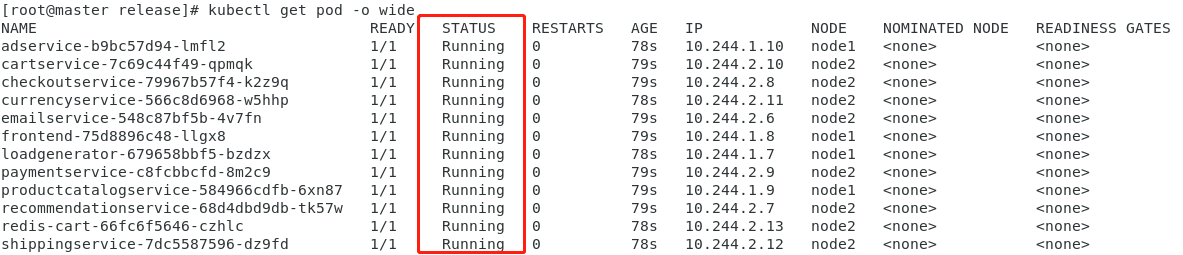
\includegraphics[width=1\textwidth]{figures/chapter2/nodes.png}
	\caption{Kubernetes资源pod列表}
	\label{fig:2-Kubernetes资源pod列表}
\end{figure}

\subsection{为微服务启用Istio支持}
进入了 `microservices-demo` 目录,并在 `istio-manifests` 目录中找到了 Istio 相关的 YAML 文件。通过使用 `kubectl apply` 命令,并指定 YAML 文件的路径,我们在集群中创建了 Istio 相关的资源,如 ServiceEntry、Gateway 和 VirtualService。使用以下命令创建了 Istio 资源:
\begin{lstlisting}[language=bash]
[root@master microservices-demo]# pwd
/root/online-boutique/microservices-demo

[root@master microservices-demo]# ls istio-manifests/
allow-egress-googleapis.yaml  frontend-gateway.yaml  frontend.yaml

[root@master microservices-demo]# kubectl apply -f ./istio-manifests
\end{lstlisting}
最后,我们获取了入口网关的 IP 地址并在浏览器中打开前端服务:
\begin{lstlisting}[language=bash]
[root@master microservices-demo]# INGRESS_HOST="$(kubectl -n istio-system get service istio-ingressgateway -o jsonpath='{.status.loadBalancer.ingress[0].ip}')"

[root@master microservices-demo]# echo "$INGRESS_HOST"

[root@master microservices-demo]# kubectl get service -n istio-system istio-ingressgateway -o wide
\end{lstlisting}

\subsection{访问首页与功能验证}
我们使用 `kubectl` 命令获取 Istio Ingress Gateway 的 IP 地址,并将其保存在 `INGRESS\_HOST` 变量中。然后,打印出该变量的值,以便在浏览器中使用。最后,使用 `kubectl get service` 命令获取 Istio Ingress Gateway 的详细信息,包括端口映射和所在节点等。在浏览器中打开 `INGRES\_HOST`,看到前端服务。在浏览器地址栏中输入 `http://<INGRESS\_HOST>/`,即可访问在线精品应用的前端界面。
删除 frontend-external 服务。frontend-external 服务是一个 LoadBalancer 服务,它暴露了前端。由于正在使用 Istio 的入口网关,不再需要这个 LoadBalancer 服务了。删除frontend-external服务,运行:
\begin{lstlisting}[language=bash]
[root@master ~]# kubectl get svc | grep frontend-external
frontend-external       LoadBalancer   10.102.0.207     192.168.110.191   80:30173/TCP   4d15h

[root@master ~]# kubectl delete svc frontend-external
service "frontend-external" deleted

[root@master ~]# kubectl get svc | grep frontend-external
\end{lstlisting}
Online Boutique 应用清单还包括一个负载发生器,它正在生成对所有服务的请求——这是为了让我们能够模拟网站的流量。
\begin{figure}[htb]
	\centering
	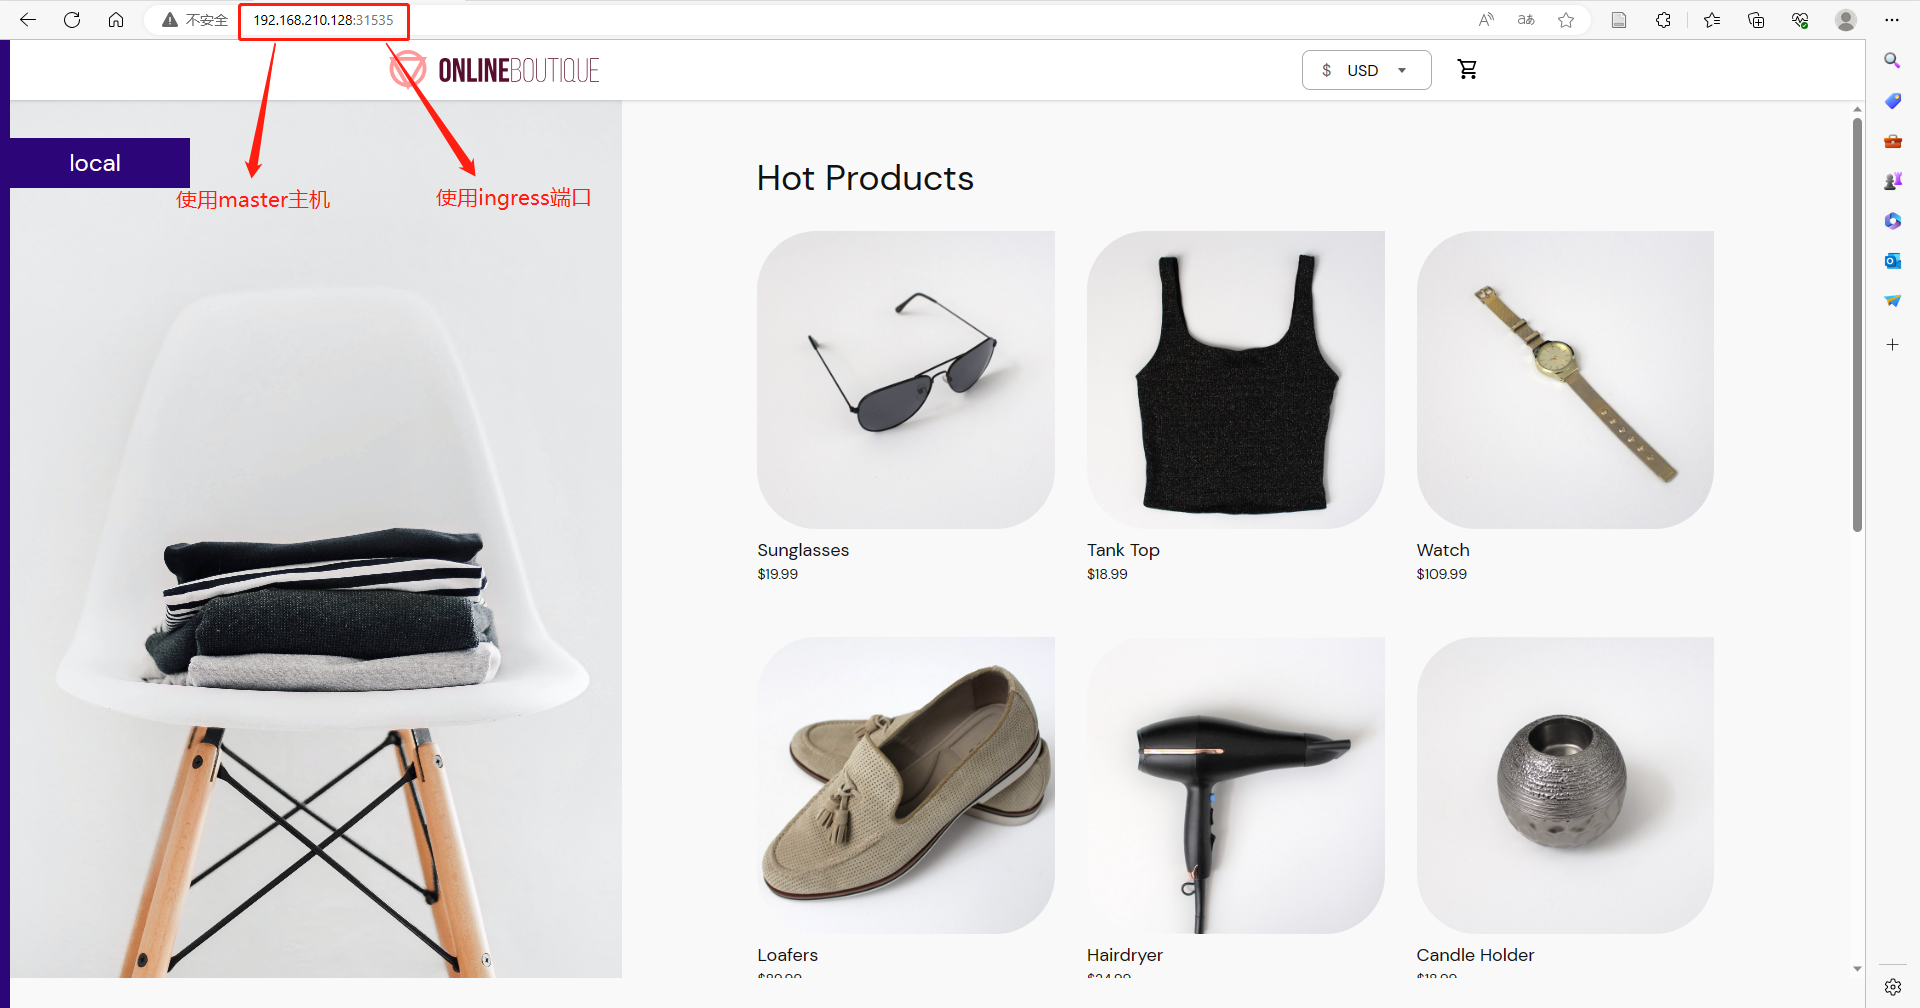
\includegraphics[width=1.0\textwidth]{figures/chapter2/Online Boutique.png}
	\caption{Online Boutique前端界面,使用ingress入口网关访问}
	\label{fig:2-Online Boutique前端界面}
\end{figure}
在Kubernetes Dashboard中查看online boutique命名空间下的服务,以adservice为例:
\begin{figure}[htb]
	\centering
	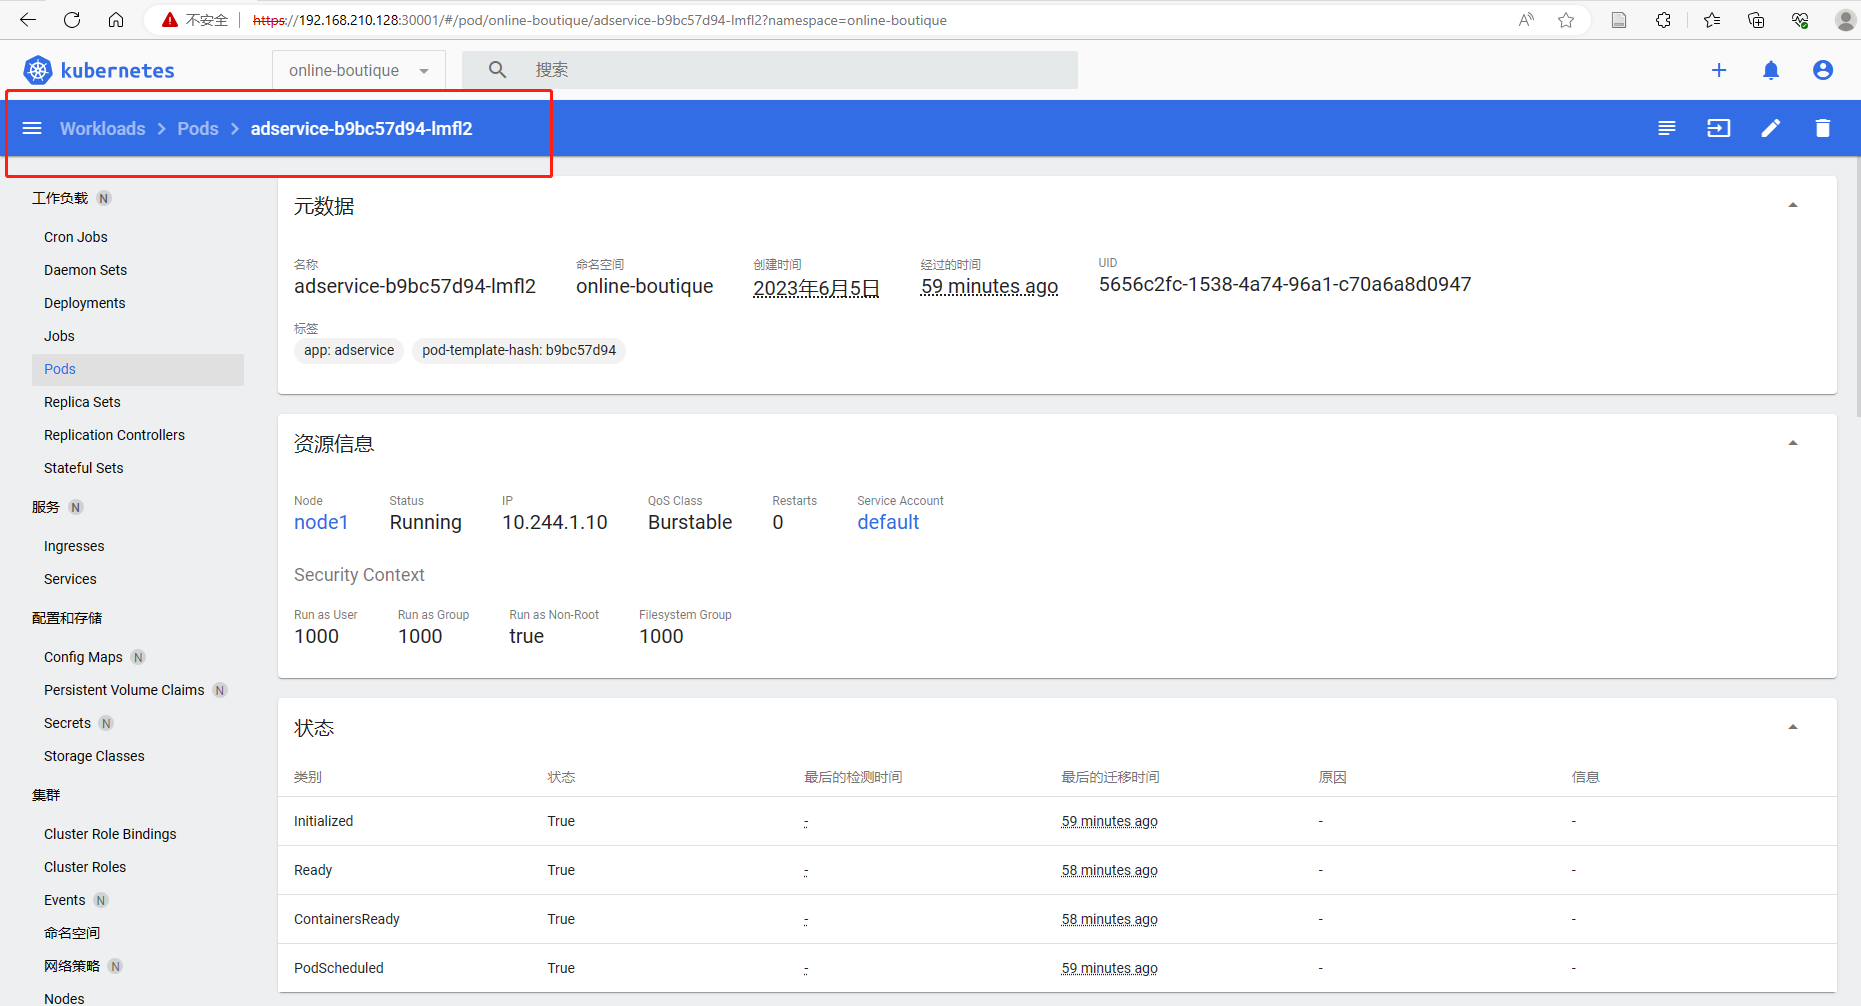
\includegraphics[width=1.0\textwidth]{figures/chapter2/online boutique on dashboard.png}
	\caption{online boutique命名空间下的服务,以adservice为例}
	\label{fig:2-online boutique命名空间下的服务,以adservice为例}
\end{figure}
